
\section{Local Vertical Local Horizontal} \label{sec:lvlh} 
Overall crew vehicle guidance, control, navitagion and communications a standard for defining vehile attitudes is usually described based on the standard Euler angle sequence for a space vehicle roll, pitch, and yaw from a 0,0,0 Local Vertical/Local Horizontal (LVLH) coordinate system as in figure \ref{fig:9}. It is possible to pick, roll yaw pitch, pitch yaw roll, pitch roll yaw, yaw roll pitch, or yaw pitch roll as the Euler sequence.

\textbf{Coordinate Frame:} Vehicle-Centered

\begin{itemize}
\item X-axis: Completes a standard, right-handed coordinate frame and is positive in the direction of vehicle motion.
\item Y-axis: Defined as a line that is normal to the orbit plane, positive in the direction opposite to the instantaneous orbit angular momentum vector.
\item Z-axis: Defined as a line that lies along the radius vector from the central body center to the vehicle center-of-mass and is positive toward the central body center.
\end{itemize}

\begin{figure}[htp]
\centering
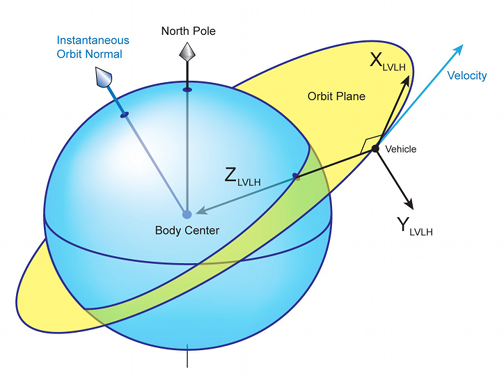
\includegraphics [width=7in]{figs/fig9.png}
\caption{LVLH}
\label{fig:9}
\end{figure}


\subsection{Example LVLH}

See the following JEOD models for an example, \hypermodelref{ORIENTATION} and \hypermodelref{DERIVEDSTATE}.


